%!TEX root = ../thesis.tex

\chapter{Results}
\label{chap:r}

\textit{[Chapter intro to be written.]}

\section{Input assessment}
\label{sec:input}

\textit{[Section intro to be written.]}

\textit{[Text below copied from P2; to be adapted.]}

In terms of datasets, both the commercial implementation and the proposed research rely on the following three sources:

\begin{itemize}
\item Nationaal Wegenbestand (NWB, National Road Database)
\item Actueel Hoogtebestand Nederland (AHN, Current Dutch Elevation)
\item Digitaal Topografisch Bestand (DTB, Digital Topographic Database)
\end{itemize}

As mentioned in the section about research questions, I am also planning to examine how specific datasets from individual NDW data suppliers (such as municipalities, road authorities, civil engineering agencies) can be integrated in the procedure and how they affect the accuracy. At this stage in the project, the specific datasets have not been selected yet.

\subsection{Nationaal Wegenbestand – NWB}
\label{sub:nwb}

\textit{[Subsection to be written.]}

\textit{[Text below copied from P2; to be adapted.]}

\begin{figure}[h]
    \centering
    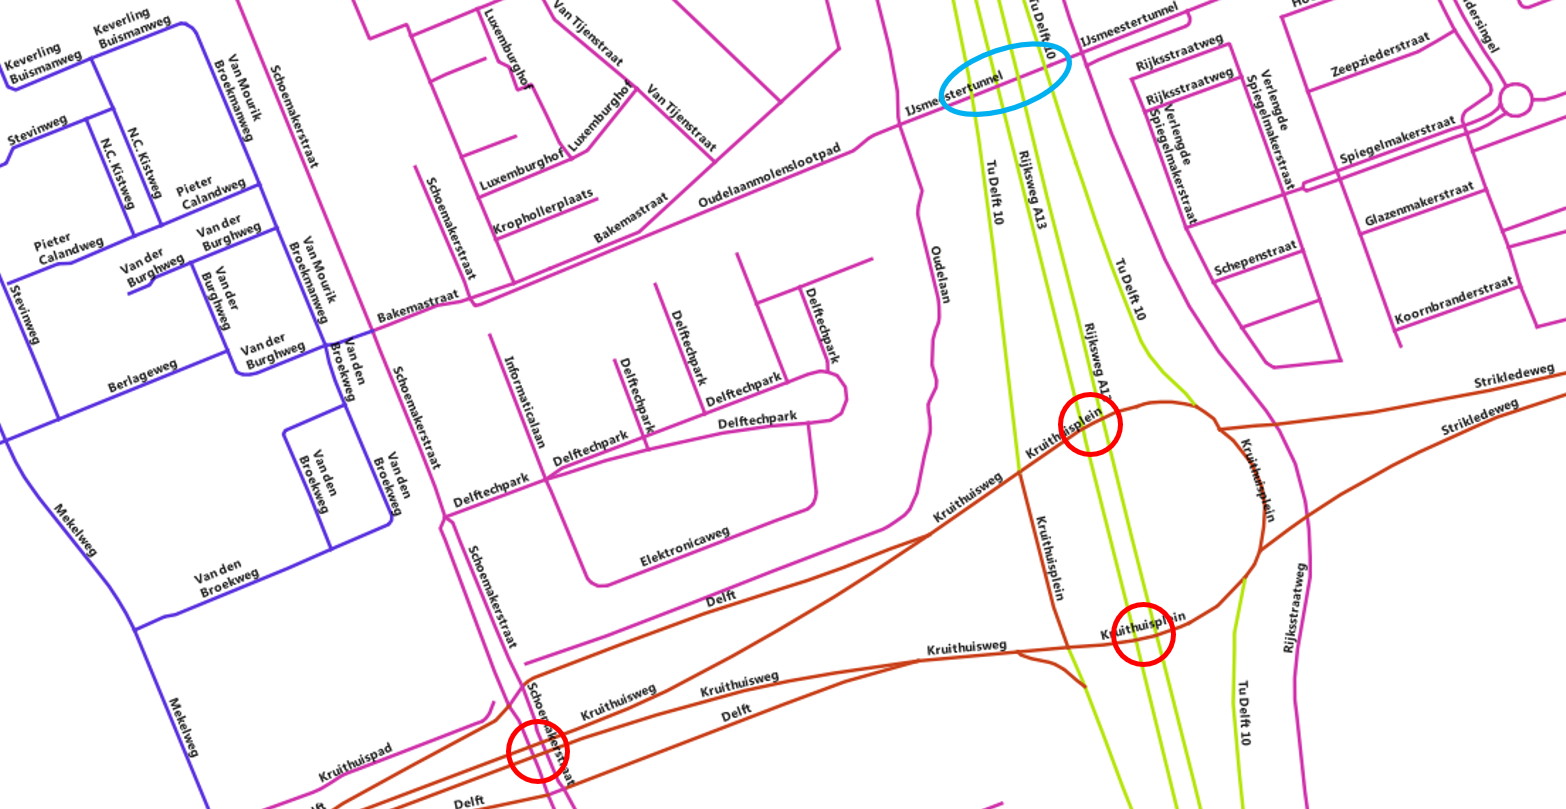
\includegraphics[width=\linewidth]{p2/figs/nwb_sample_02.png} 
    \caption{An example render of NWB. The road segments \textit{(wegvakken)} are colour-coded to indicate management \textit{(wegbeheerdersoort)}. Yellow is used for R-roads (state-managed roads), red denotes P-roads (province-managed roads), magenta means G-roads (municipality-managed roads), and W-roads (RWS-managed roads) are not shown in this figure. Blue roads (T-roads) are roads which do not fall into the above 4 categories, in this case they are managed by TU Delft. This render also contains examples of challenging 3D relationships. Where the P-road Kruithuisweg/Kruithuisplein crosses the G-road Schoemakerstraat and the R-road A13, no intersection occurs in 2D because the roads cross over one another in 3D. These locations are indicated in the figure by red circles. Furthermore, where the bike path IJsmeestertunnel (a G-road in NWB) crosses the A13, a series of 3 short tunnels are located in reality. This is indicated in the figure by a blue oval. These are two types of road layouts that we expect to have to dedicate special attention to.}
    \label{fig:nwb}
\end{figure}

NWB (or more specifically, NWB-Wegen, the NWB roads product) is an \textit{ESRI Shapefile}-based vector dataset comprised of a semantically rich set of 2D \textit{MultiLineString} objects. They are interconnected in such a way that NWB can be regarded topologically as a graph representation of the Dutch road network. Although the NWB contains all named and numbered roads in The Netherlands, we are only interested in roads that are semantically marked as state-owned or province-owned (category R for Rijk and P for Provincie), because the new noise regulation is only relevant to these types. NWB and the road types it contains are illustrated in Figure \ref{fig:nwb}. In addition to its important topological graph structure, the NWB lines are georeferenced with good accuracy. Although the accurate nature of its georeferencing is specifically mentioned in the documentation of the data, it is not evidenced by a rigorous evaluation. The quality description includes only a single figure, which is 5-metre accuracy at two standard deviations (i.e. 95\% confidence), but with the confidence being based on the total number of roads, implying that the accuracy evaluation method is performed on a road-to-road basis, each of which may be comprised of multiple \textit{MultiLineString} objects. It is not described, how the accuracy is evaluated for each road, for instance whether it is based on the accuracy of the vertex locations of the road, an arbitrary sampling along their length, and how it is aggregated. Furthermore, we do not know whether the reference for the accuracy was empirical (surveyed control points) or whether it is purely theoretical and is based on the sources and the methods involved in creating  and updating the dataset. Both the topological and the geographical information content of NWB is assembled from a wide range of providers ranging from large national providers such as RWS and Kadaster, to local providers such as specific road authorities and civil engineering agencies. No clear indication is given in the documentation about the sources used for the compilation of specific NWB road types or the estimation of their accuracies, but it is mentioned that they are inconsistent across the range of road types (\cite{nwb_docs}). Although the above nominal lateral accuracy (and its description) is not sufficient for compliance with the new noise regulations, the 3D conversion of NWB is not concerned with improving it – in fact, it is a requirement of the project not to displace NWB horizontally. Hence, we may say that the intended outcome of the 3D conversion is to devise a method that can produce accurate elevations for NWB assuming it  is up to SWUNG2 standards. To achieve this in practice, lateral refinement is being done in a separate project by developing a workflow to match NWB roads with roads in another Dutch national open data geospatial dataset called Basisregistratie Grootschalige Topografie (BGT). Since BGT is already compliant with the accuracy requirements, correcting NWB geometries based on BGT will foreseeably solve the lateral accuracy problem of NWB. However, at the time of writing of this report, the BGT-based correction has only been carried out and released for municipality-owned roads (category G for Gemeente), hence both the commercial and the scientific 3D-NWB project still rely on NWB data that lacks this correction (\cite{nwb_gecorrigeerd}). Regardless of improving NWB’s lateral accuracy not being within the scope of this project, it is important to be aware of the uncertainty because of its implications when overlaying NWB with other datasets, such as AHN and DTB.

\begin{figure}[ht]
    \centering
    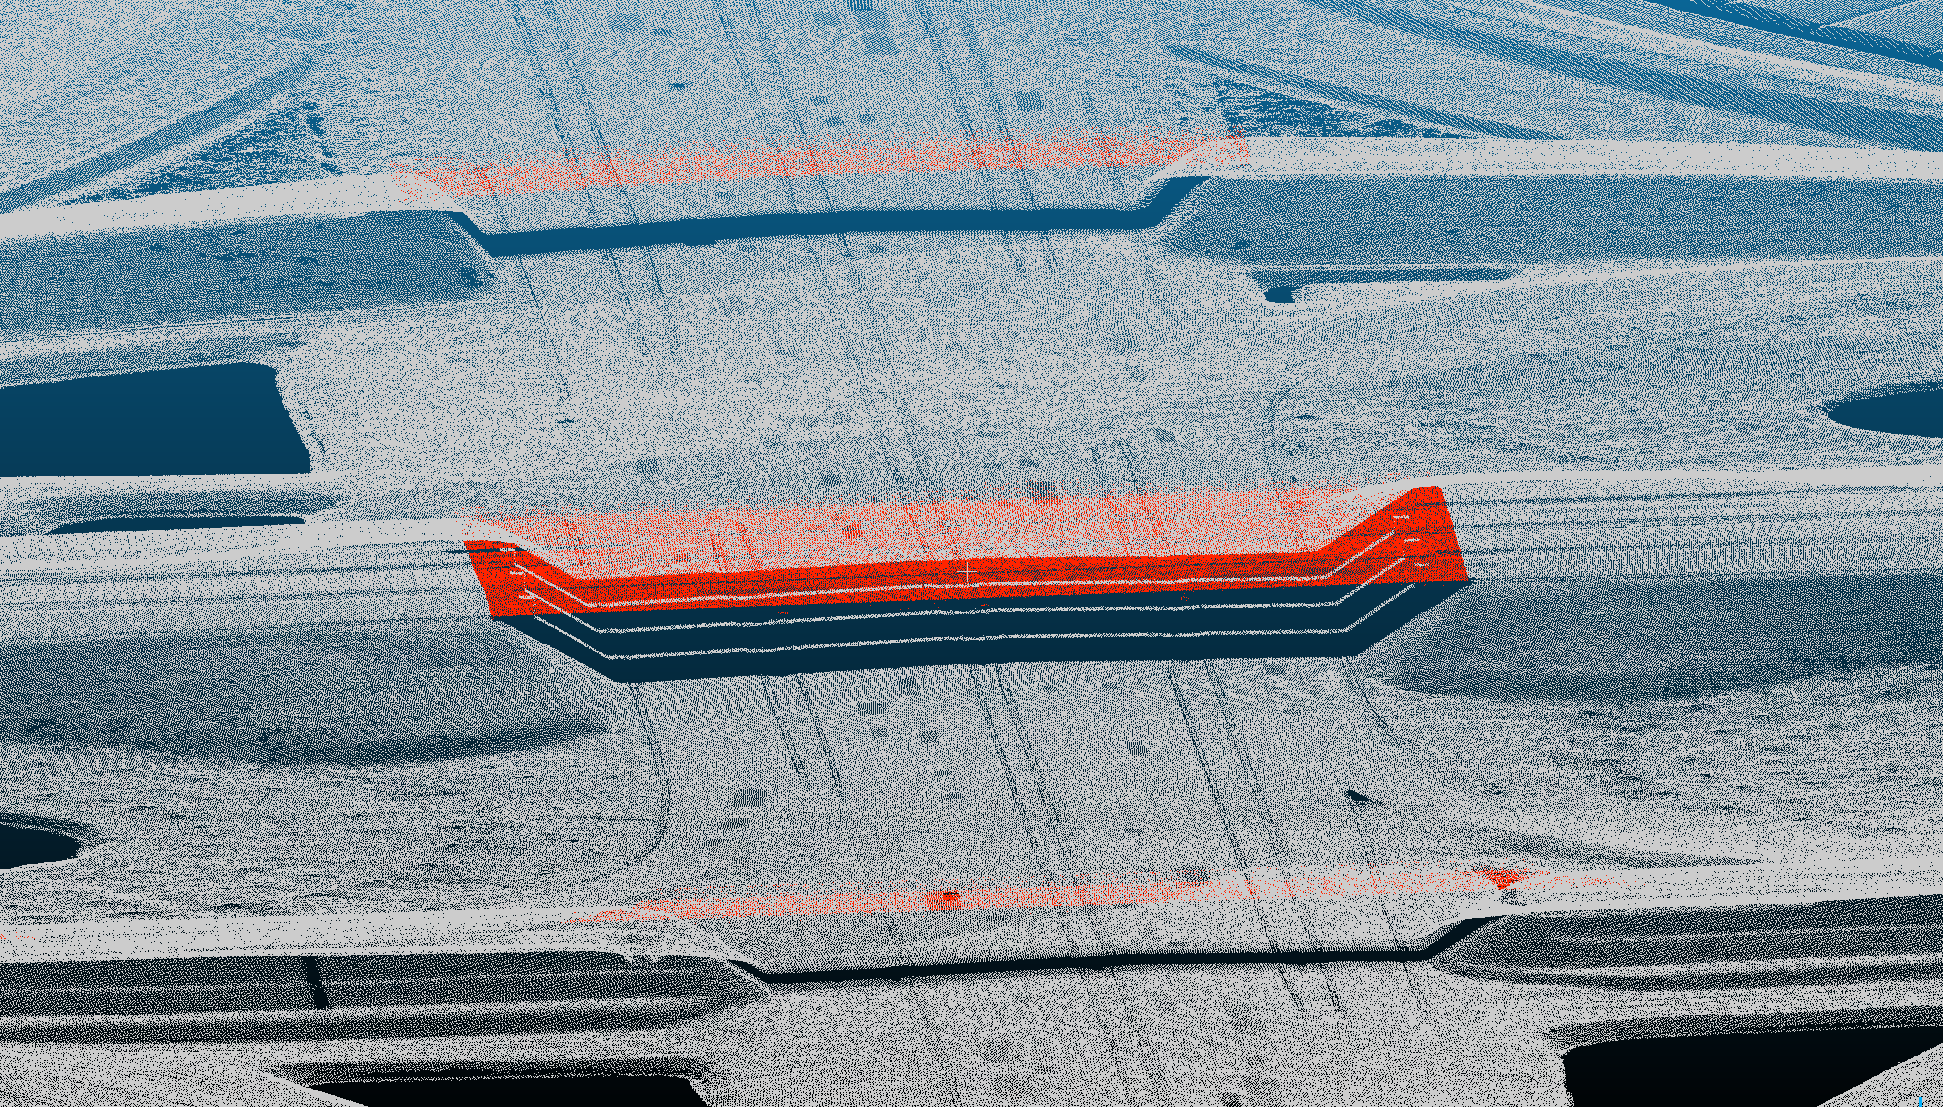
\includegraphics[width=\linewidth]{p2/figs/ahn_sample_01.png} 
    \caption{An example render of AHN3 with the original point density (no thinning applied) at the Knoppunt Deil, SW of Geldermalsen. The white colour corresponds to ground points (class 2), red corresponds to bridges (class 26). All other classes were removed. The shapes of motorway lanes and ramps, as well as bridges are clearly defined. Road constructed on elevated ground is reliably classified as ground, bridges are cleanly split off by the classification. Even under thin bridges, data becomes gradually sparser at the border and becomes extinct directly below the bridge. This render also makes it clear that wherever vehicles were encountered, the sampling is worse locally. It does not go entirely extinct however, as most locations have been scanned multiple times.}
    \label{fig:ahnbridges}
\end{figure}

\subsection{Actueel Hoogtebestand Nederland – AHN}
\label{sub:ahn}

\textit{[Subsection to be written.]}

\textit{[Text below copied from P2; to be adapted.]}

AHN are airborne Lidar (ALS) survey datasets available as open government geospatial data in The Netherlands. The surveys are commissioned every few years with AHN1 to AHN3 already complete (1996 to 2019), and the first AHN4 surveys nearing release. At this stage of the project, we are interested in AHN3, although it is a planned side-track of the research to examine how freshly released AHN4 data could best be made use of. The dataset has a combined systematic and stochastic elevation error of 15 centimetres at two standard deviations (i.e. 95 \% confidence), and 6 to 10 points per square metre point density on average, corresponding to a 0.41 to 0.32 metre posting distance. The lateral error is 18 centimetres at two standard deviations (\cite{ahn_kwaliteit}). Comparing these to the descriptors of datasets mentioned in research examined as part of our literature review (see the Relevant work section), AHN3 can be considered accurate, and to have excellent point density. The AHN3 point cloud has been classified semi-automatically with great accuracy and is released with the classification included. This means that for most purposes, the point cloud needs not be ground filtered manually, and that extracting certain features is made far easier. Of the various classes available, we are interested in class 2 the most, which corresponds to ground points, and class 26 which contains, among other things, bridges. Ground points are primarily interesting to us because they contain the road points. This includes roads that were constructed directly on the terrain, as well as roads constructed on altered terrain, such as those built on elevated ground or in open trenches. It also contains the points that represent the terrain in the vicinity of the roads. Elevated roads and bridges are not considered ground points and are generally represented by gaps in class 2, which can, in most cases, be filled by using data from class 26, as shown in Figure \ref{fig:ahnbridges}. However, it is worth noting that class 26 also contains other types of objects, for instance large motorway signs arching over the road surface (shown in Figure \ref{fig:ahnsigns}), as well as the civil engineering structures of elevated roads and bridges (in addition to the road surfaces on them).
\begin{figure}[h!]
    \centering
    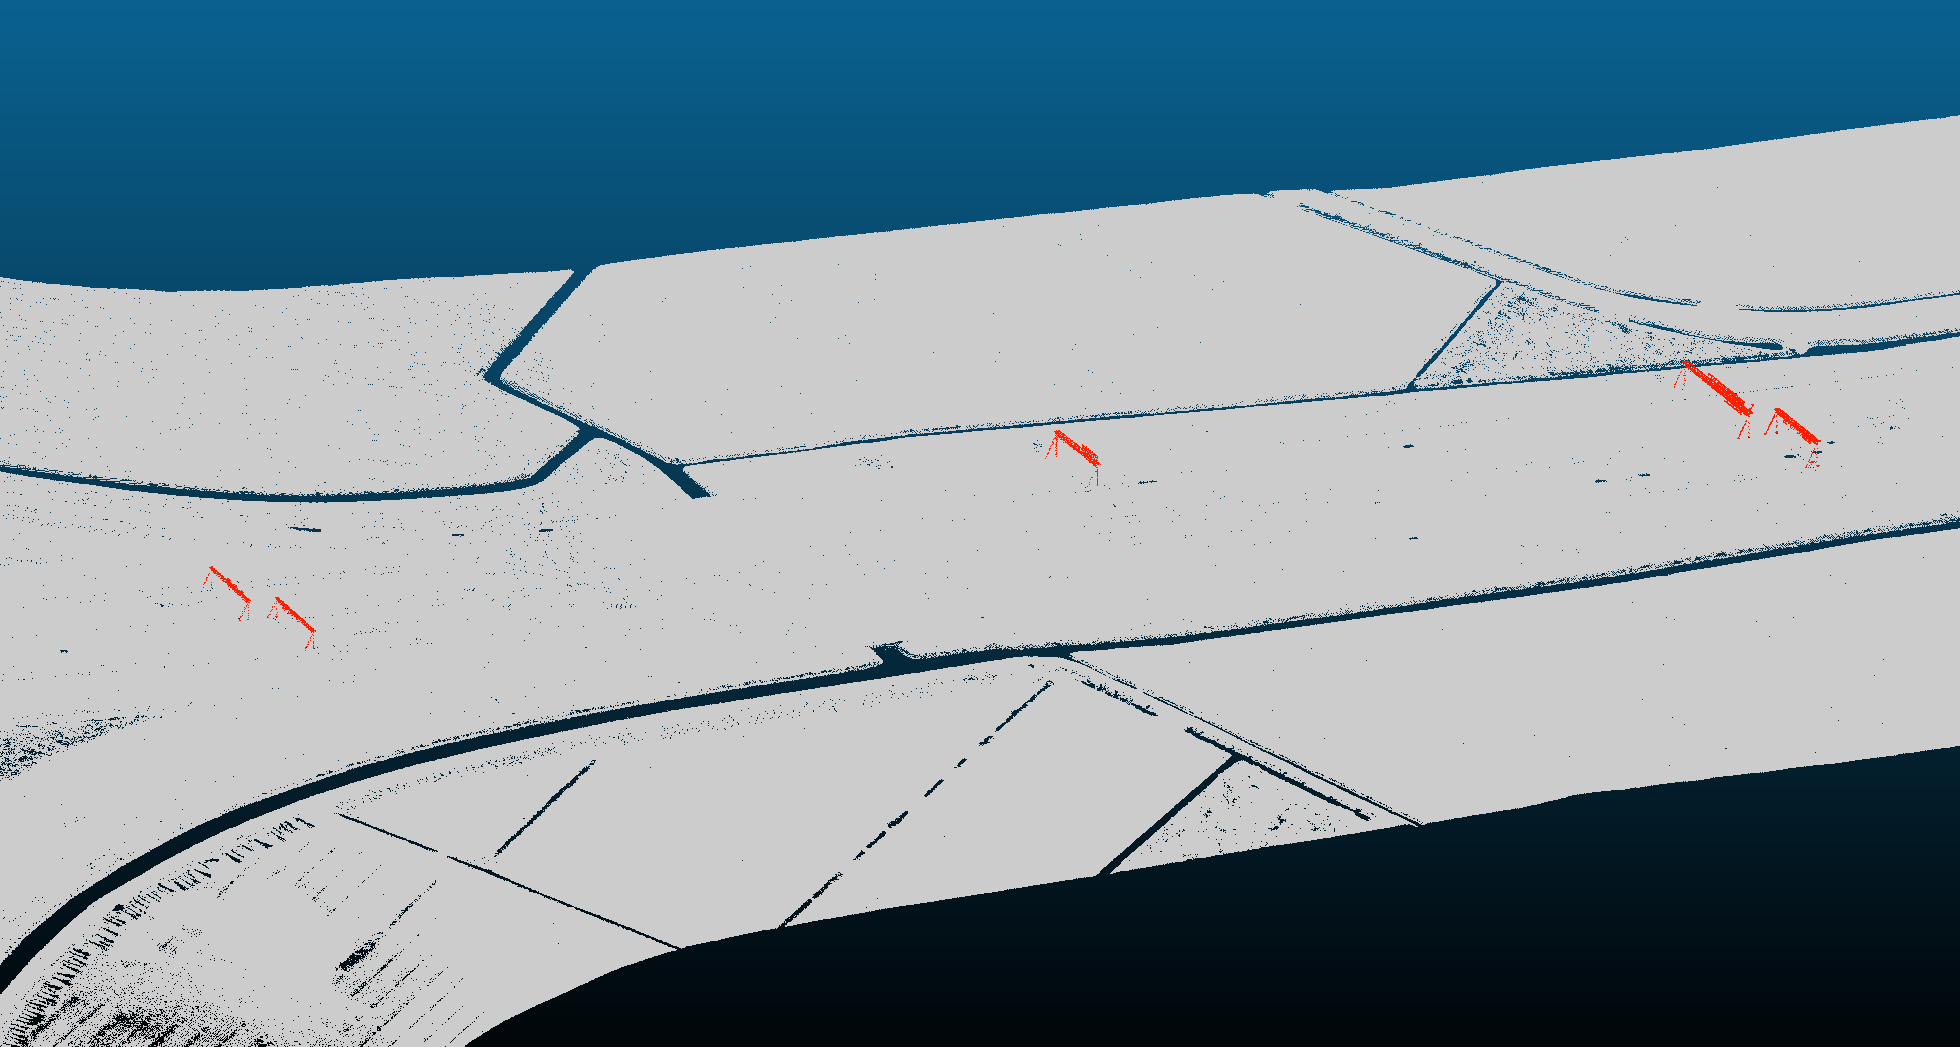
\includegraphics[width=\linewidth]{p2/figs/ahn_sample_02.png} 
    \caption{This render is from the same location and data as \ref{fig:ahnbridges}. Here it is visible that my testing datasets, all points falling outside a 150-metre buffer zone around the NWB centrelines have been removed. While class 26 primarily contains bridges, this image shows that full-width motorway signs are also contained by it. It also shows that the presence of water results in holes (the dark, linear features running parallel with the motorway in this render) in the ground-only point cloud.}
    \label{fig:ahnsigns}
\end{figure}
\begin{figure}[h!]
    \centering
    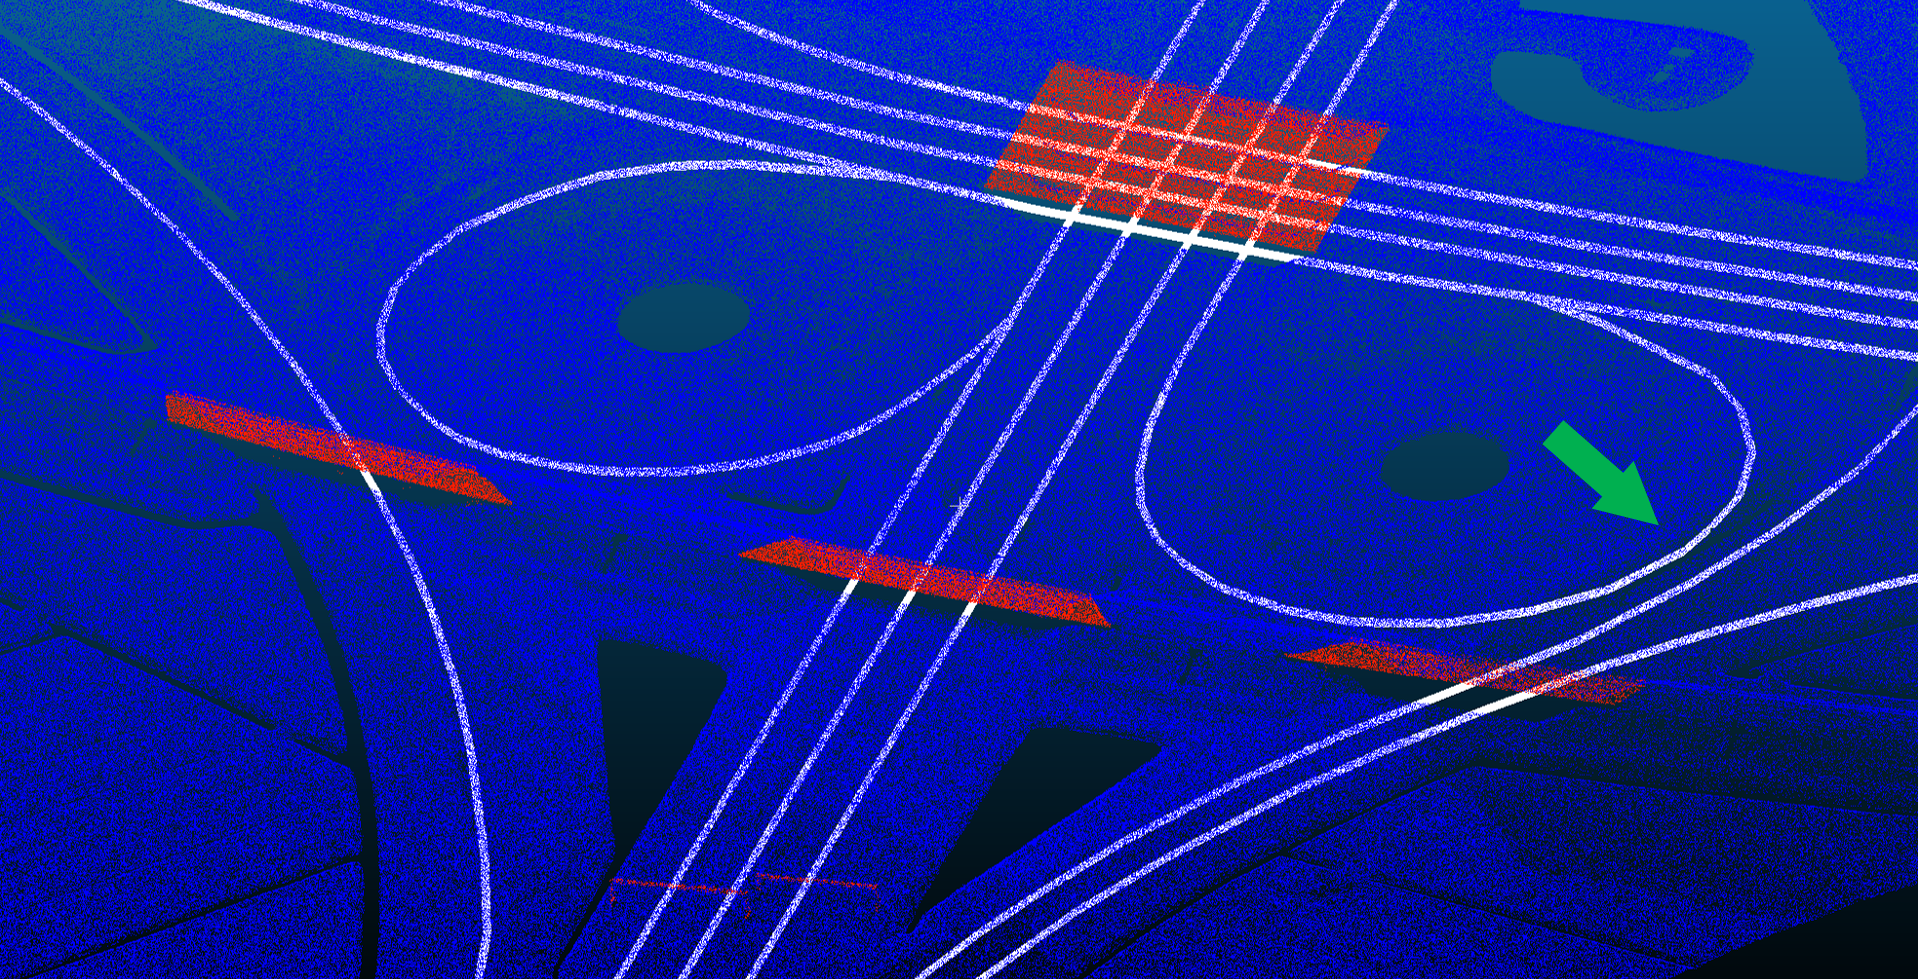
\includegraphics[width=\linewidth]{p2/figs/ahn_sample_04_a.png} 
    \caption{This render is from the same location and data as Figures \ref{fig:ahnbridges} and \ref{fig:ahnsigns}. Here, ground points are coloured blue, and NWB centrelines are shown in white. As they have no elevation, they appear below AHN3 points and are consequently masked out partially by them. In general, the visual agreement between AHN3 and NWB appears to be good. The most noticeable deviations from the AHN3-defined centrelines of roads occur where they are intensely curved, and where motorway ramps merge into motorway lanes. The reason for the prior appears to mostly be the angularity introduced by the finite discretisation of curves in NWB, for instance in the location pointed out by the green arrow. The succession on three bridges in the bottom of the image do not have an associated NWB centreline because they are railway bridges. The same would be observed for roads not yet registered in NWB (i.e. newly roads).}
    \label{fig:ahnnwb}
\end{figure}
AHN3 is released in the form of a point cloud, as well as DSM and DTM rasters. Both DEMs were produced using basic radial IDW interpolation with a fixed parametrisation. The DTM was generated by including only points from class 2 in the interpolation step. They are available at 0.5-metre and 5-metre resolutions, with the 0.5-metre resolution being relevant to this project in terms of the target accuracy. For context, this raster converts (on average) 1.5 to 2.5 points into a single raster cell. The Lidar tiles are released in the binary LAZ format (compressed LAS, or LASzip), and are generally several gigabytes in size. As each tile only covers an approximate area of 32 square kilometres and the LAZ compression ratio for this dataset is 0.1 on average, scaling considerations are relevant to this project.

\begin{figure}[h!]
    \centering
    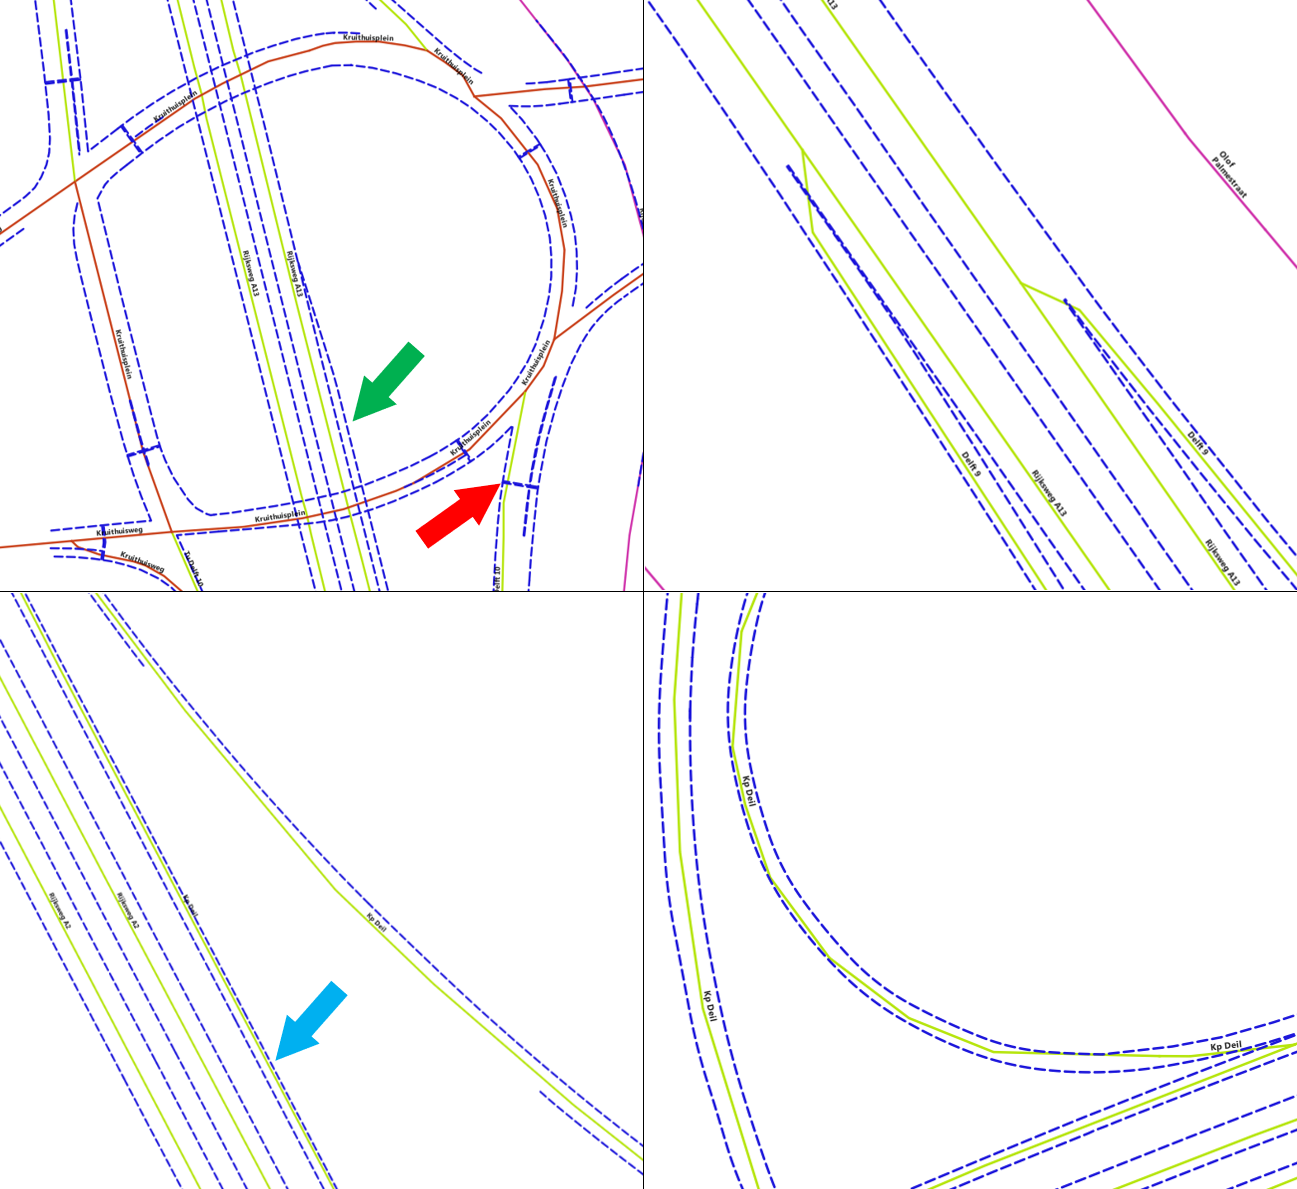
\includegraphics[width=0.95\linewidth]{p2/figs/dtb_sample_07.png} 
    \caption{Renders of DTB \textit{verflijnen} overlaid with NWB centrelines, illustrating "compatibility issues" and individual DTB issues. NWB symbology is identical to the one used in \ref{fig:nwb}, blue dashed lines are the DTB lines. \textbf{Top left:} there is not necessarily only one \textit{verflijnen} line on either side of NWB (green arrow). Furthermore, stop lines are also often in this category. \textbf{Top right:} NWB motorway ramps often merge with the motorway lanes at unrealistic angles. This causes NWB to intersect DTB lines at these locations. \textbf{Bottom left:} DTB road edges are often missing. Furthermore, NWB centrelines may be very close to DTB edges, as indicated by the blue arrow. \textbf{Bottom right:} NWB discretisation and inaccuracy often results in angular lines in sharp bends. NWB often gets close to, even intersects DTB in such places. Although this is a 2D visualisation, DTB has 3D geometry as Figure \ref{fig:dtbahn} illustrates.}
    \label{fig:dtbnwb}
\end{figure}

\subsection{Digitaal Topografisch Bestand – DTB}
\label{sub:dtb}

\textit{[Subsection to be written.]}

\textit{[Text below copied from P2; to be adapted.]}

\begin{figure}[h!]
    \centering
    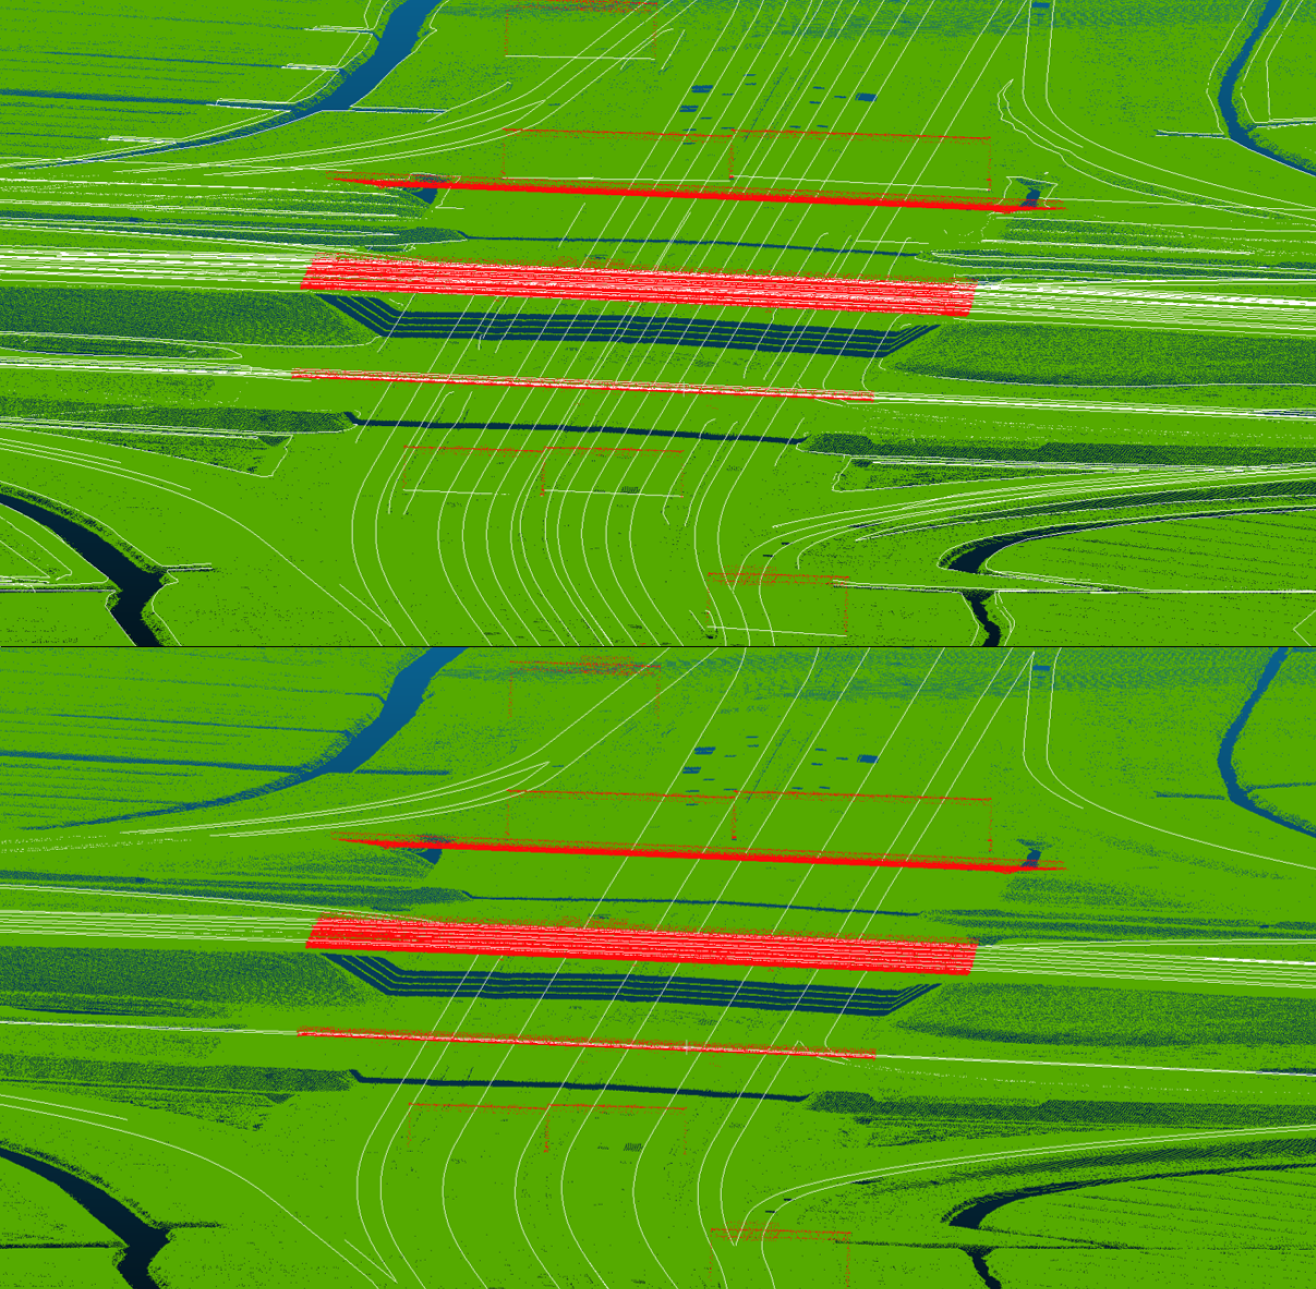
\includegraphics[width=0.95\linewidth]{p2/figs/ahn_sample_10.png} 
    \caption{Renders of DTB line features overlain with AHN3 in 3D. Ground points are shown in green. \textbf{Top:} all DTB lines are shown, illustrating that other features, such as roadside slopes, canals, ditches, safety rails are represented in DTB. Full-width motorway signs are occasionally represented (either by lines on the road, or on the structure itself, inconsistently). \textbf{Bottom:} Only \textit{verflijnen} shown. The lines are generally in good agreement with AHN3 visually. This figure also illustrates that they may be useful for identifying which class-26 Lidar points lie on road surfaces, as they contain good first approximations for their elevations.}
    \label{fig:dtbahn}
\end{figure}

Like NWB, DTB (or more specifically, DTB-Droog, the DTB roads product) is a Dutch open data geospatial dataset in the \textit{ESRI Shapefile} format. For the purposes of this project, we only need DTB street outlines (edges), hence we can also regard this as a dataset comprised exclusively of \textit{MultiLineString} objects, making it identical to NWB in its data structure. DTB is managed by RWS and it is concerned only with state-owned roads and roads on state-leased land, which translate almost exclusively to NWB R-roads. DTB is, hence, not a reliable source of information about provincial roads (NWB P-roads), our other road type of interest. The DTB lines that are commonly used as road edges are not, in fact, the edges of the paved surface. They are called \textit{verflijnen}, and are the approximate locations of the painted lines representing the outermost edges of the area open to traffic. This is a lucky correspondence with NWB, as it too, contains the centrelines of the areas of roads that are open to traffic. The second-best option would be to use the category \textit{gelederail constructie}, which generally provide good approximations of the edges of the paved surfaces on which the \textit{verflijnen} were painted. Unfortunately, these correspond to the location of safety rails, and as such they are sometimes not on the road and are also not always present. Like NWB (but unlike AHN), DTB’s acquisition also concerns several organisations performing various types of sensing, which are then semi-automatically assembled into the complete DTB product. DTB lines are primarily photogrammetry-derived, with land-based surveying methods and car-mounted Lidar (MLS) used in some areas to improve accuracy (\cite{oudeElberink_vosselman_2012}). The documentation of DTB consist of a documentation (\cite{dtb_docs}) and a handbook (\cite{dtb_handbook}). The accuracy of DTB is not published by RWS or any other organisation contributing to or using the dataset, although it is generally thought to be quite accurate. It is mostly used for purposes relating to road management and civil engineering and apart from road edges, it contains more than 400 other types of semantically identified roadside object types. As most users of DTB work in GIS environments, particular care is taken to separate objects into layers in such a way that inside any one layer, they never overlap. This means that they can be processed using 2D GIS tools easier, reducing the significance of elevation to a mere semantic detail (non-geometric attribute). Whenever objects in any given such layer are found in the same position (or closer than a certain threshold), they are automatically shifted by a maximum distance of 5 centimetres to eliminate the overlap, most commonly for DTB road signs. While descriptions in the documentation can be found suggesting that DTB lines are measured accurately, I must consider the formal accuracy of DTB unknown due to the lack of any numerical figures or other evidence to support this. Furthermore, as I illustrate in \ref{fig:dtbnwb}, a visual comparison with NWB reveals various types of significant inconsistencies and interpretation issues. A visual comparison with AHN3 is also shown in \ref{fig:dtbahn}.

\subsection{Testing datasets}
\label{sub:testingdata}

\textit{[Subsection to be written.]}

\textit{[Text below copied from P2; to be adapted.]}

Due to its volume, it will not be possible to develop and test the implementation without cropping AHN3 input point cloud tiles. Even after the implementation of the segmentation workflow, the size of the testing point clouds will need to be manageable, to facilitate efficient debugging. At the same time, they will need to be representative enough to provide an insight into the computational complexity and visual performance of the algorithm. I have already produced a range of testing datasets by selecting various lengths of NWB centrelines at interesting road features, and keeping only those Lidar points which are within a 150-metre buffer distance from the selected road centrelines. Table \ref{tab:inventory} provides an inventory of these. The tile identifier in the first column refers to those used in \cite{ahn3_download}. The resulting datasets fit into memory easily, even when extracted to LAS.

\begin{longtable}[c]{@{}p{2.8cm}p{6.8cm}c@{}}
\toprule
Title, tile  & Features & Render \\ \midrule
Markerwarddijk, 20BN1 & Dike-based P-road in the Markermeer. Very limited amount of terrain around the road. Road consistently build on ground, with no involvement of bridge structures. & \raisebox{-0.94\totalheight}{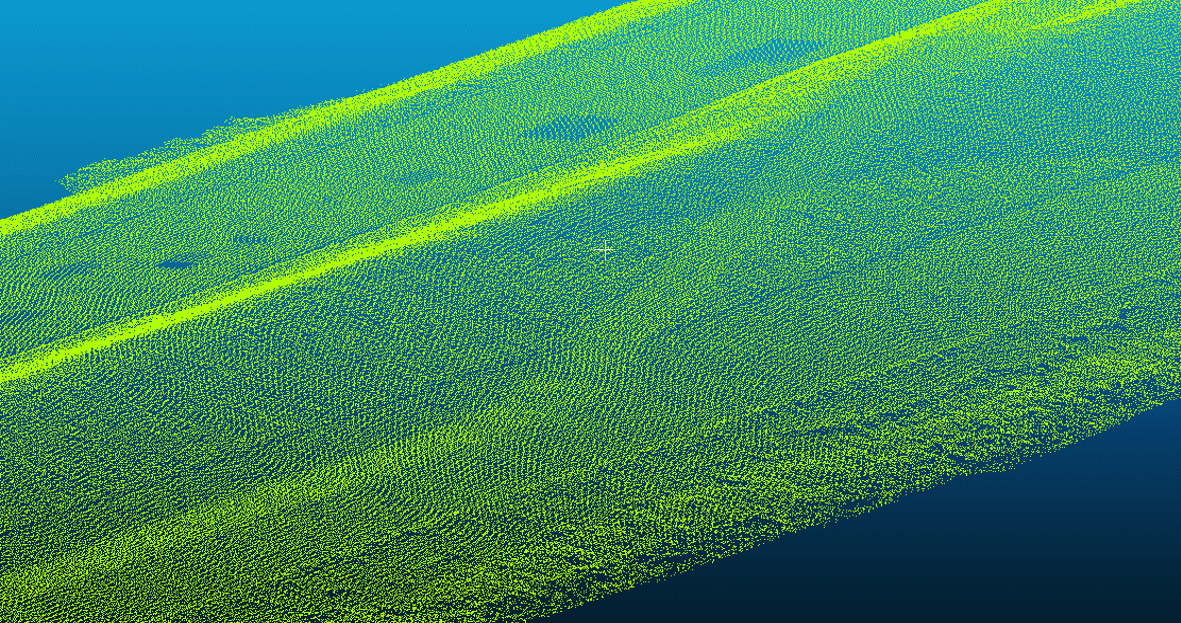
\includegraphics[width=6cm, height=3.5cm]{p2/figs/ahn_sample_20BN1_a.png}}  \\
Amsterdam Hemhavens, 25BZ2 & Ringweg-West (R-road) as it crosses the IJ through the Coentunnel in a densely built-up environment. It is built on artificially elevated ground and on bridges in this area. Part of Westradweg also included, which has been built entirely on a long bridge. & \raisebox{-0.94\totalheight}{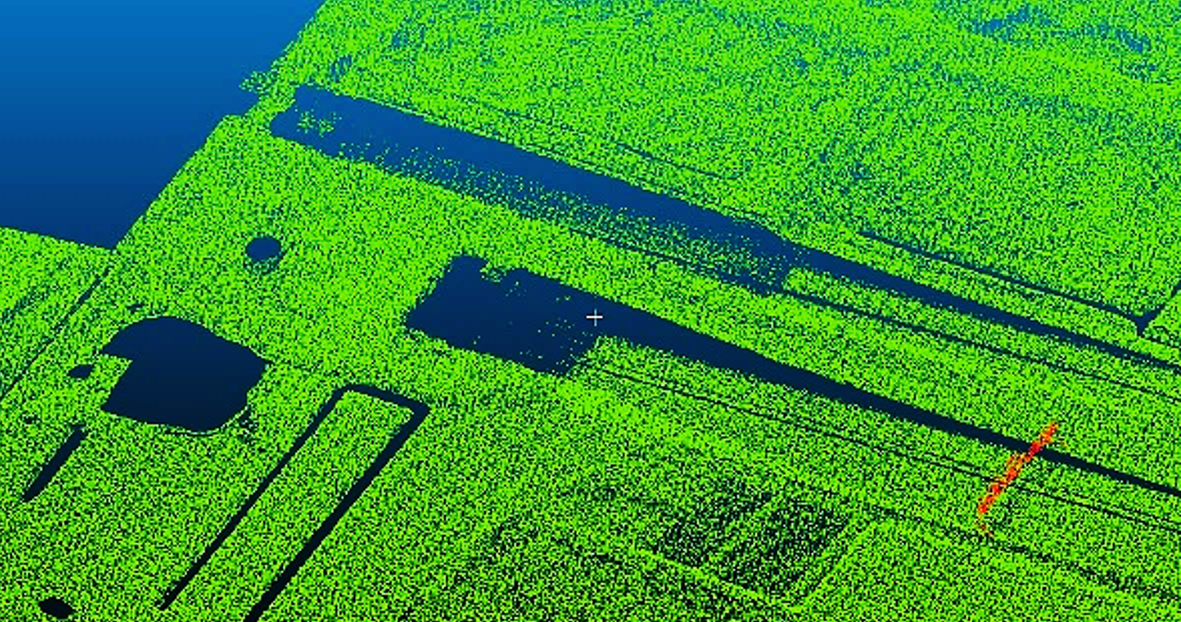
\includegraphics[width=6cm, height=3.5cm]{p2/figs/ahn_sample_25BZ2_a.png}} \\
Amsterdam Zuid, 25DN2 & R-roads with many closely spaced bridges, small tunnels, dense grouping of holes around roads due to presence of water and buildings & \raisebox{-0.94\totalheight}{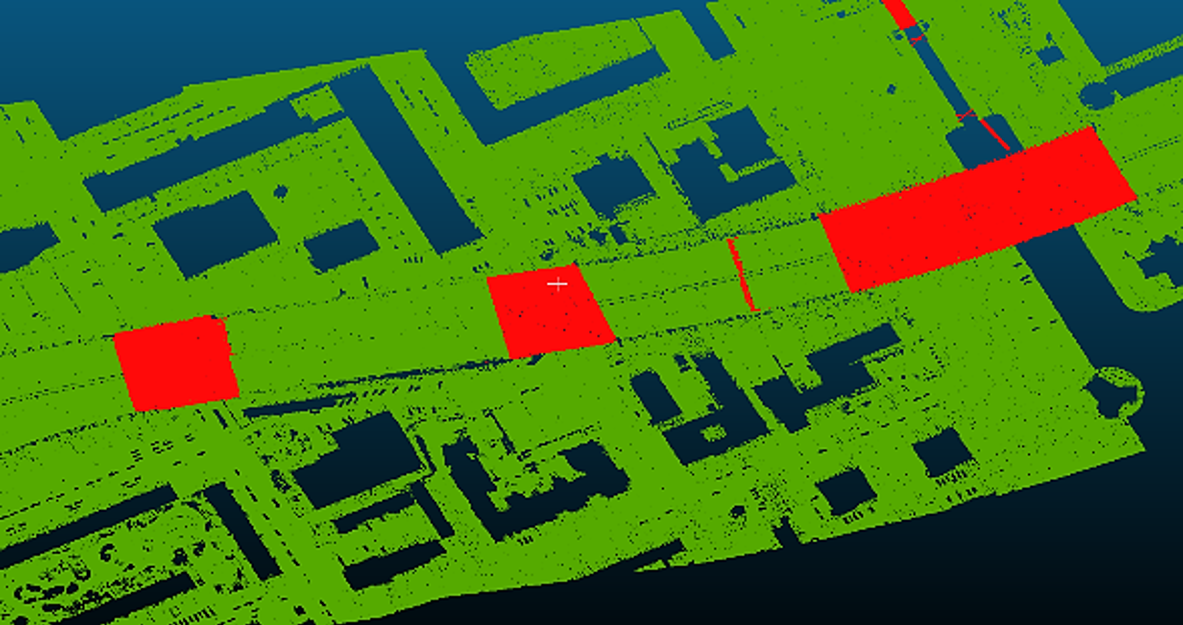
\includegraphics[width=6cm, height=3.5cm]{p2/figs/ahn_sample_25DN2_a.png}} \\
Bunschoten, 32BN1 & P-roads with three big roundabouts, and one road that ends in a small roundabout. Amersfoortseweg has its two lanes on separate roads surfaces (like motorways), but with frequent connecting segments. & \raisebox{-0.94\totalheight}{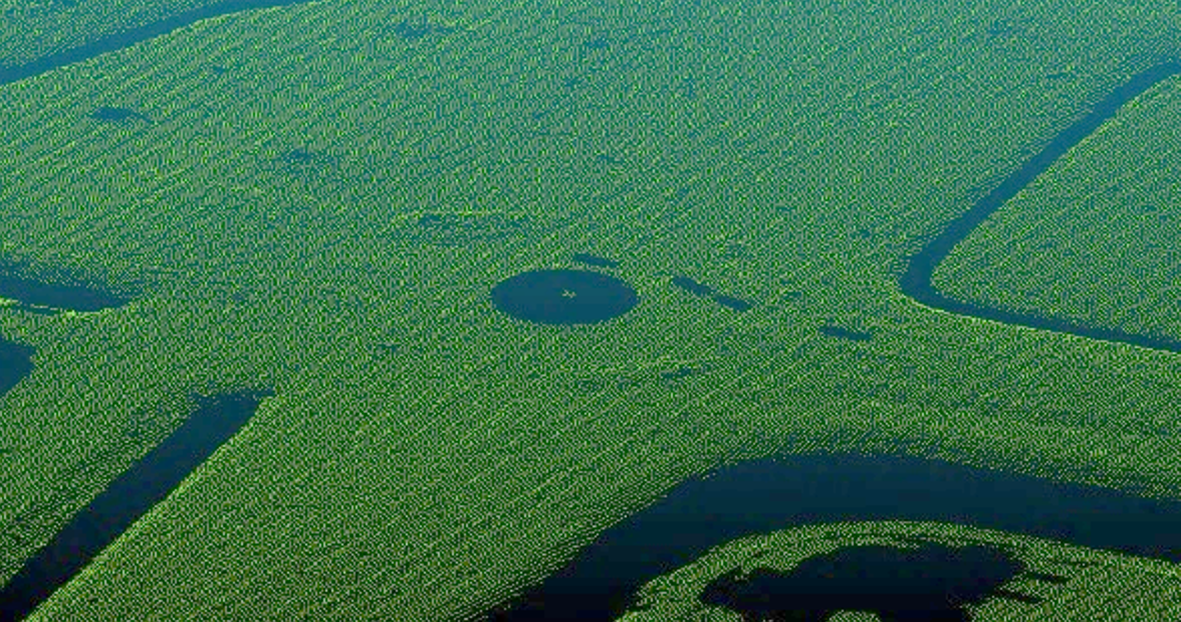
\includegraphics[width=6cm, height=3.5cm]{p2/figs/ahn_sample_32BN1_a.png}} \\
Veluwe, 32FZ2 & Straight R-roads surrounded by dense forest and crossed by wide wildlife overpasses. & \raisebox{-0.94\totalheight}{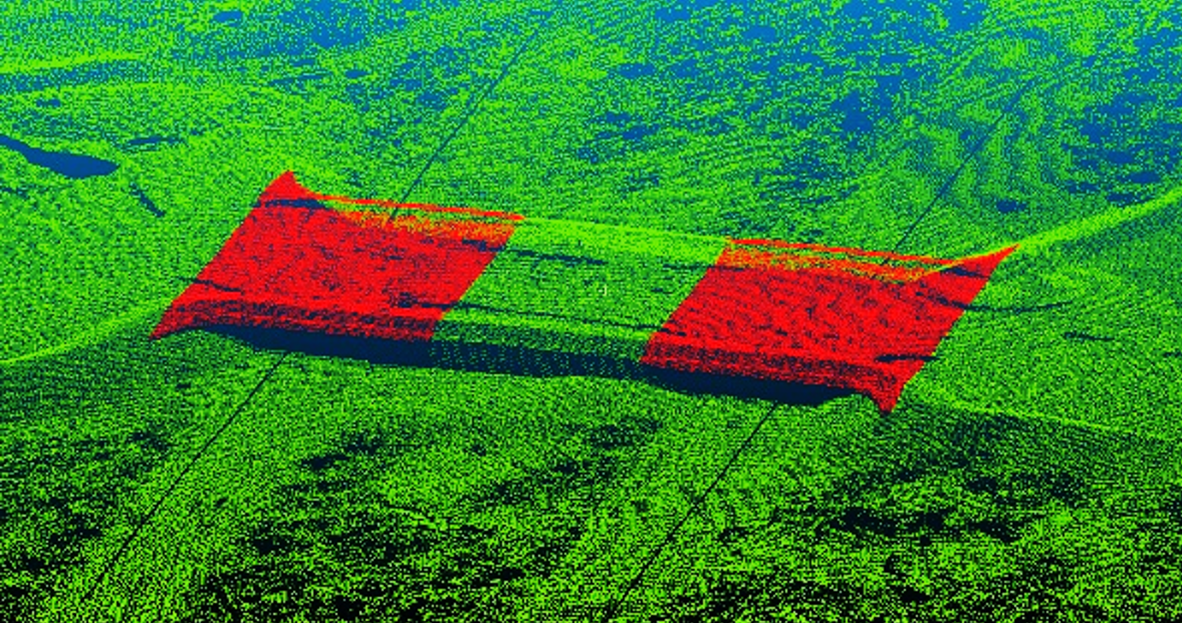
\includegraphics[width=6cm, height=3.5cm]{p2/figs/ahn_sample_32FZ2_a.png}} \\
Apeldoornseweg, 32HZ2 & P-road in dense forest with canopy frequently occluding the road surface, decreasing point density and occasionally creating gaps. The road has small parallel branches running very close to it, which may make it difficult for the algorithm to distinguish between them. It also has roundabouts. & \raisebox{-0.94\totalheight}{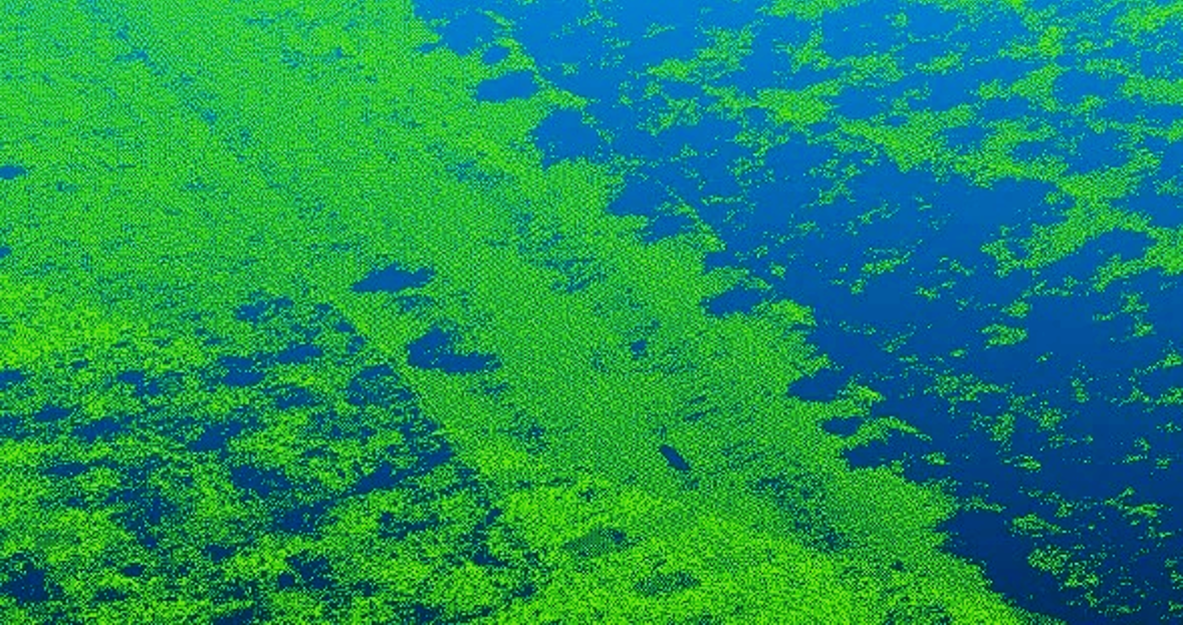
\includegraphics[width=6cm, height=3.5cm]{p2/figs/ahn_sample_32HZ2_a.png}} \\
Hoenderloo, 33CN2 & P-road in extremely dense, continuous forest with canopy frequently occluding the road surface, decreasing point density and occasionally creating gaps. Both lanes are on the same road surface & \raisebox{-0.94\totalheight}{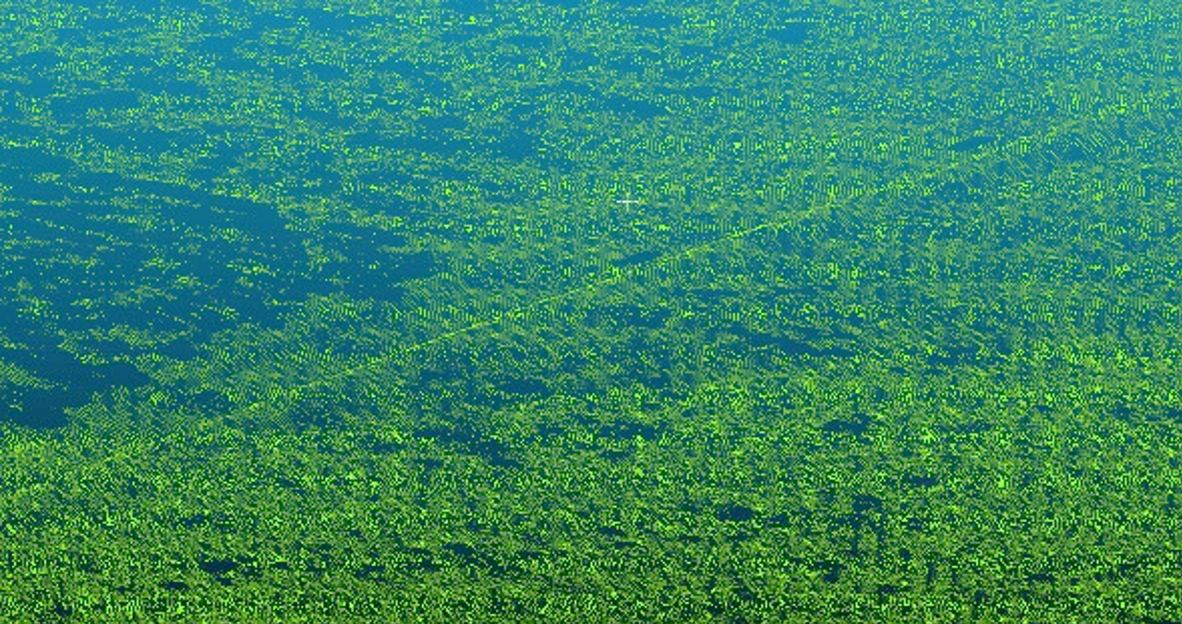
\includegraphics[width=6cm, height=3.5cm]{p2/figs/ahn_sample_33CN2_a.png}} \\
Rotterdam Ketheltunnel, 37EZ1 & This segment of the A4 heading North from Rotterdam has been recently reconstructed in an underground tunnel. In addition, a significant portion of this R-road now runs in a trench towards Delft. AHN3 was imaged during the reconstruction, and hence contains erratic data about the road surface. & \raisebox{-0.94\totalheight}{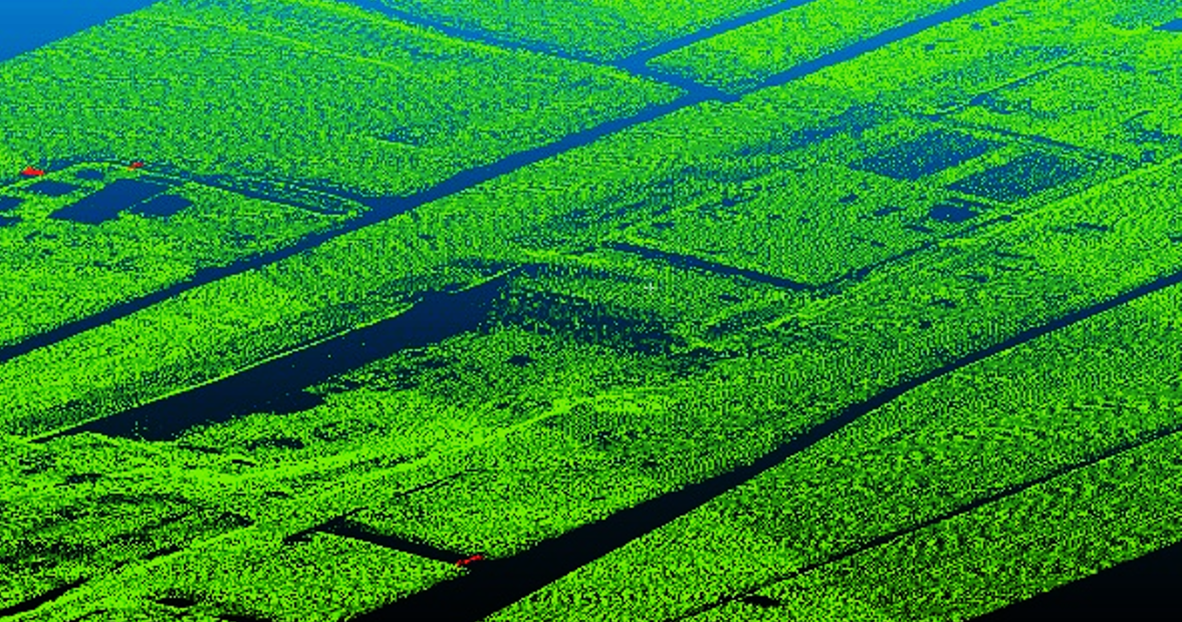
\includegraphics[width=6cm, height=3.5cm]{p2/figs/ahn_sample_37EZ1_a.png}} \\
Knoppunt Ridderkerk, 37HN2 & The Ridderkerk interchange is one of the largest of its kind in The Netherlands, in one place containing 4 overlapping R-roads. Furthermore, it contains an extremely high density of R-roads in a small area, many of them very tightly packed in small areas. Many are intensely curved. & \raisebox{-0.94\totalheight}{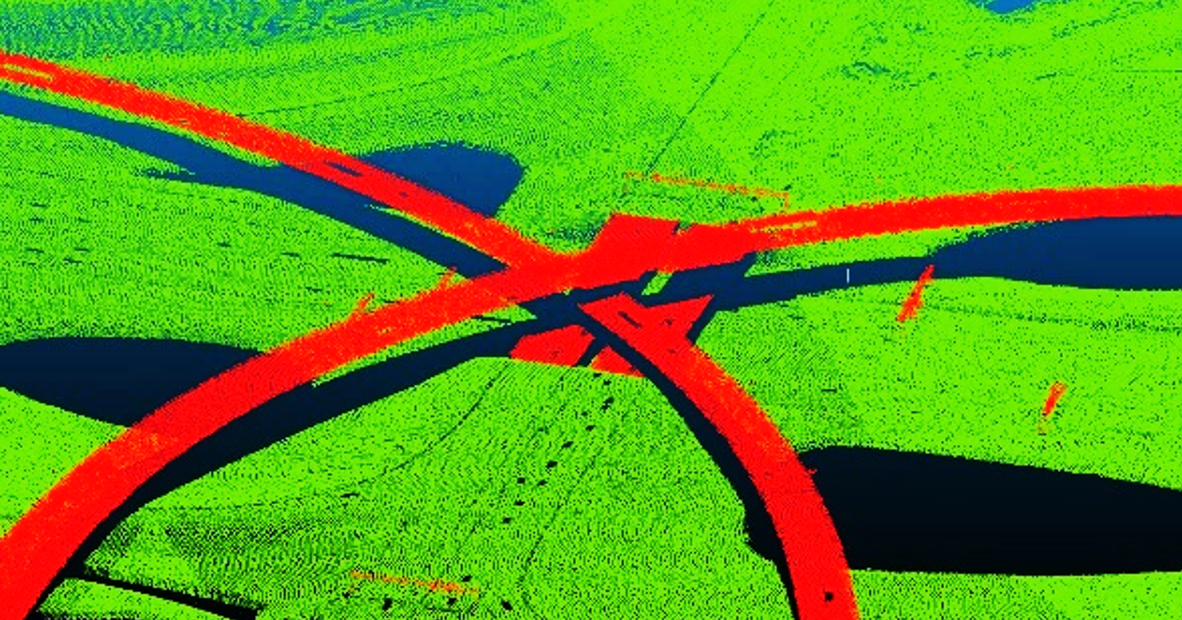
\includegraphics[width=6cm, height=3.5cm]{p2/figs/ahn_sample_37HN2_a.png}} \\
Gorinchem, 38GZ1 & Complex interchange between a P-road and an R-road with small ramps, roundabouts and overlapping geometries. & \raisebox{-0.95\totalheight}{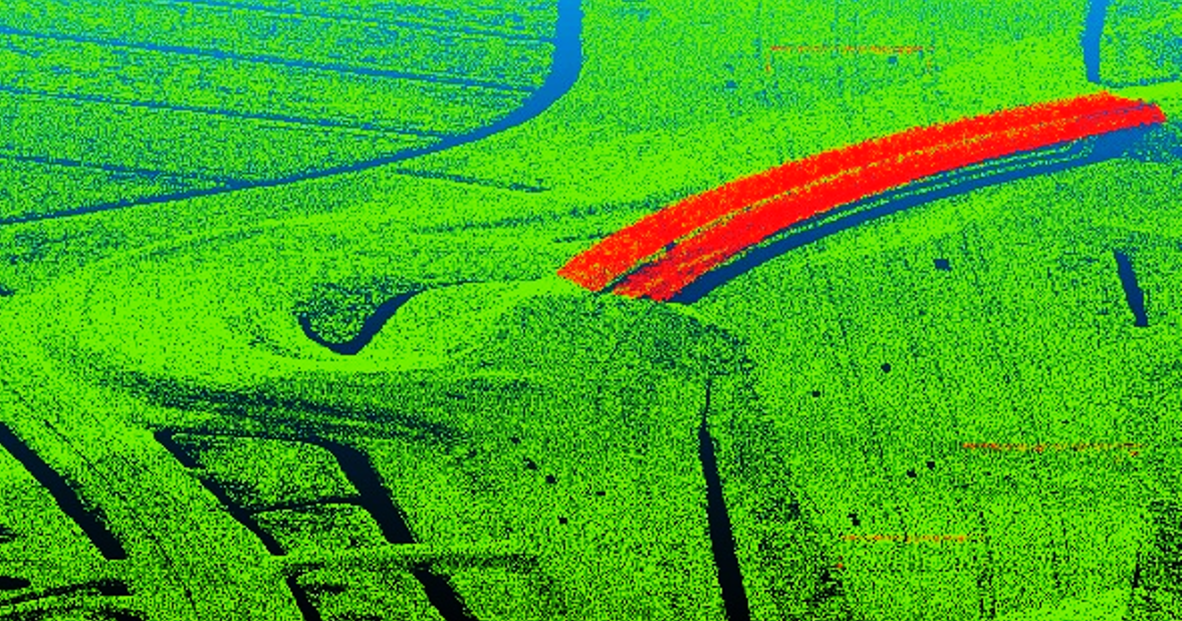
\includegraphics[width=6cm, height=3.5cm]{p2/figs/ahn_sample_38GZ1_a.png}} \\
Knoppunt Deil, 39CZ1 & Less complex, but analogous interchange to the Knoppunt Ridderkerk. & \raisebox{-0.5\totalheight}{\textit{Please refer to Figures \ref{fig:ahnbridges}, \ref{fig:ahnsigns}, \ref{fig:ahnnwb} and \ref{fig:dtbahn}.}} \\
\toprule
\caption{Inventory of testing datasets \label{tab:inventory}}
\end{longtable}

\section{Results of processing steps}
\label{sec:results}

\textit{[Section intro to be written.]}

\subsection{Splitting NWB into NBRS}
\label{sub:r_nbrsgeneration}

\textit{[Subsection to be written.]}

\subsection{Lidar segmentation}
\label{sub:r_lidarsegmentation}

\textit{[Subsection to be written.]}

\subsection{Edge approximation}
\label{sub:r_edgeapproximation}

\textit{[Subsection to be written.]}

\subsection{Active contour optimisation}
\label{sub:r_activecontours}

\textit{[Subsection to be written.]}

\subsection{TIN construction}
\label{sub:r_tinconstruction}

\textit{[Subsection to be written.]}

\subsection{Interpolation in TIN and snapping}
\label{sub:r_interpolation}

\textit{[Subsection to be written.]}

\section{Accuracy assessment}
\label{sec:accuracy}

\textit{[Section intro to be written.]}

\subsection{Which steps affect accuracy?}
\label{sub:accuracysteps}

\textit{[Subsection to be written.]}

\subsection{TIN completeness and accuracy}
\label{sub:accuracytin}

\textit{[Subsection to be written.]}

\subsection{3D road network accuracy}
\label{sub:accuracynwb}

\textit{[Subsection to be written.]}

\section{Comparison with commercial implementation}
\label{sec:comparison}

\textit{[Section intro to be written.]}

\subsection{Overall comparison}
\label{sub:comparisonoverall}

\textit{[Subsection to be written.]}

\subsection{R-roads}
\label{sub:comparisonrroads}

\textit{[Subsection to be written.]}

\subsection{P-roads}
\label{sub:comparisonproads}

\textit{[Subsection to be written.]}